\documentclass[8pt]{extarticle}
\title{}
\author{}
\date{}
\usepackage[shortlabels]{enumitem}


%paper setup
\usepackage{geometry}
\geometry{letterpaper, portrait, margin=1in}
\usepackage{fancyhdr}
% sans serif font:
\usepackage{cmbright}
%symbols
\usepackage{amsmath}
\usepackage{bigints}
\usepackage{amssymb}
\usepackage{amsthm}
\usepackage{mathtools}
\usepackage[hidelinks]{hyperref}
\usepackage{gensymb}
\usepackage{multirow,array}
\usepackage{multicol}

\newtheorem*{remark}{Remark}
\usepackage[T1]{fontenc}
\usepackage[utf8]{inputenc}

%chemistry stuff
%\usepackage[version=4]{mhchem}
%\usepackage{chemfig}

%plotting
\usepackage{pgfplots}
\usepackage{tikz}
\tikzset{middleweight/.style={pos = 0.5}}
%\tikzset{weight/.style={pos = 0.5, fill = white}}
%\tikzset{lateweight/.style={pos = 0.75, fill = white}}
%\tikzset{earlyweight/.style={pos = 0.25, fill=white}}

%\usepackage{natbib}

%graphics stuff
\usepackage{graphicx}
\graphicspath{ {./images/} }
\usepackage[style=numeric, backend=biber]{biblatex} % Use the numeric style for Vancouver
\addbibresource{the_bibliography.bib}
%code stuff
%when using minted, make sure to add the -shell-escape flag
%you can use lstlisting if you don't want to use minted
%\usepackage{minted}
%\usemintedstyle{pastie}
%\newminted[javacode]{java}{frame=lines,framesep=2mm,linenos=true,fontsize=\footnotesize,tabsize=3,autogobble,}
%\newminted[cppcode]{cpp}{frame=lines,framesep=2mm,linenos=true,fontsize=\footnotesize,tabsize=3,autogobble,}

%\usepackage{listings}
%\usepackage{color}
%\definecolor{dkgreen}{rgb}{0,0.6,0}
%\definecolor{gray}{rgb}{0.5,0.5,0.5}
%\definecolor{mauve}{rgb}{0.58,0,0.82}
%
%\lstset{frame=tb,
%	language=Java,
%	aboveskip=3mm,
%	belowskip=3mm,
%	showstringspaces=false,
%	columns=flexible,
%	basicstyle={\small\ttfamily},
%	numbers=none,
%	numberstyle=\tiny\color{gray},
%	keywordstyle=\color{blue},
%	commentstyle=\color{dkgreen},
%	stringstyle=\color{mauve},
%	breaklines=true,
%	breakatwhitespace=true,
%	tabsize=3
%}
% text + color boxes
\renewcommand{\mathbf}[1]{\mathbold{#1}}
\usepackage[most]{tcolorbox}
\tcbuselibrary{breakable}
\tcbuselibrary{skins}
\newtcolorbox{problem}[1]{colback=white,enhanced,title={\small #1},
          attach boxed title to top center=
{yshift=-\tcboxedtitleheight/2},
boxed title style={size=small,colback=black!60!white}, sharp corners, breakable}
%including PDFs
%\usepackage{pdfpages}
\setlength{\parindent}{0pt}
\usepackage{cancel}
\pagestyle{fancy}
\fancyhf{}
\rhead{Avinash Iyer}
\lhead{Math 400: Homework 9}
\newcommand{\card}{\text{card}}
\newcommand{\ran}{\text{ran}}
\newcommand{\N}{\mathbb{N}}
\newcommand{\Q}{\mathbb{Q}}
\newcommand{\Z}{\mathbb{Z}}
\newcommand{\R}{\mathbb{R}}
\begin{document}
  \begin{problem}{Problem 1}
    True or false: If $H$ is a minor of $G$, then $H$ is a contraction of a subgraph of $G$.
    \tcblower
    True.
  \end{problem}
  \begin{problem}{Problem 2}
    Prove each of the following.
    \begin{enumerate}[(a)]
      \item There exists an infinite family $F$ of graphs such that no graph in $F$ is a subgraph of another graph in $F$.
      \item There exists an infinite family $F$ of graphs such that no graph in $F$ is a contraction of another graph in $F$.
      \item There exists an infinite family $F$ of graphs such that no graph in $F$ is a subgraph or a contraction of another graph in $F$.
    \end{enumerate}
    \tcblower
    \begin{problem}{(a)}
      Cycles; if we delete any vertex or edge of any cycle, then the degree of at least two vertices is reduced by $1$, while all vertices in every cycle are of degree $2$.
    \end{problem}
    \begin{problem}{(b)}
      The family of graphs $K_{2,n}$:
      \begin{center}
        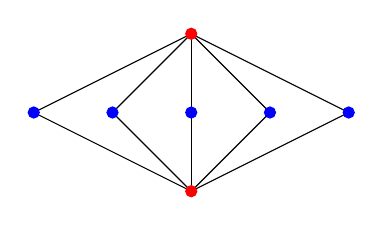
\begin{tikzpicture}
          \draw (0,1) -- (-2,0);
          \draw (0,1) -- (-1,0);
          \draw (0,1) -- (0,0);
          \draw (0,1) -- (2,0);
          \draw (0,1) -- (1,0);
          \draw (0,-1) -- (-2,0);
          \draw (0,-1) -- (-1,0);
          \draw (0,-1) -- (0,0);
          \draw (0,-1) -- (2,0);
          \draw (0,-1) -- (1,0);
          \filldraw[red] (0,1) circle (2pt)
                (0,-1) circle (2pt);
          \filldraw[blue] (-2,0) circle (2pt)
                          (-1,0) circle (2pt)
                          (0,0) circle (2pt)
                          (1,0) circle (2pt)
                          (2,0) circle (2pt);
        \end{tikzpicture}
      \end{center}
    \end{problem}
  \end{problem}
  \begin{problem}{Problem 3}
    Prove that the set of all planar graphs is minor-closed.
    \tcblower
    Let $G$ be any planar graph. Then, by Wagner's theorem, it must be the case that neither $K_{5}$ nor $K_{3,3}$ are minors of $G$. Therefore, any minor of $G$, $G'$, must also not have $K_{5}$ nor $K_{3,3}$ as a minor --- otherwise, we would take the steps to create $G'$, then the steps to create one of the forbidden minors, and $G$ would have the forbidden minors as a minor.\\

    Thus, since no minor of any planar graph can be non-planar, it must be the case that planarity is minor-closed.
  \end{problem}
  \begin{problem}{Problem 4}
    Let $P$ be an arbitrary set of graphs. Let $P'$ be the set of all graphs not in $P$. By the Graph Minor Theorem, $P$ has a finite subset $F$ of graphs that are minor-minimal in $P$. Similarly, $P'$ has a finite subset $F'$ of graphs that are minor minimal in $P'$. Prove that if $P$ is minor-closed, then a graph $G$ is in $P'$ if and only if $G$ has a minor in $F'$. So, if $P$ is minor-closed, then $P$ and $P'$ are both ``characterized'' by $F'$. In fact, if $P$ is minor-closed, then $F$ consists of only one graph, namely the graph with only one vertex. Why?
    \tcblower
    Suppose $P$ is minor-closed. Then, if $H\in F$, then no minor of $H$ is in $P$ or $F$. 
    \begin{description}
      \item[$(\Rightarrow)$] Let $G\in P$. Suppose toward contradiction that there is a graph $H\in F'$ that is a minor of $G$.\\

        Since $P$ is minor-closed, and $H$ is a minor of $G\in P$, $H\in P$.\\

        However, $H\in F'\subseteq P'$. So, $H\in P$ and $H\in P'$. $\bot$
      \item[$(\Leftarrow)$] Suppose that no graph in $F'$ is a minor of $G$. Suppose toward contradiction that $G \notin P$.\\

        Then, $G\in P'$.\\

        So, by definition of $F'$, $G$ must have a minor in $F'$.\\

        So, $\exists H\in F'$ such that $H$ is a minor of $G$. $\bot$
    \end{description}
    Since any graph that is in $F$ must have a minor that is also in $F$, every graph in $F$ must reduce to the graph of one vertex.
  \end{problem}
  \begin{problem}{Problem 5}
    A graph $G$ is apex if $G-v$ is planar for some vertex $v$ of $G$. Prove that the set of apex graphs is minor-closed.
    \tcblower
    Let $G$ be an apex graph --- we will show that any minor of $G$ must also be apex.
  \end{problem}
  \begin{problem}{Problem 6}
    Prove that if $G$ is a connected graph, then for every edge $e$, $G-e$ has at most two connected components.
    \tcblower
    Let $e = ab$.\\

    If $G-e$ is connected, then we are done. Otherwise, if $G-e$ is not connected, $\exists v,w\in V(G-e)$ such that there is no path in $G-e$ from $v$ to $w$.\\

    Since $G$ is connected, $\exists$ a path $P = (v,v_1,\dots,a,b,\dots,v_n,w)$ in $G$. It must be the case that $e\in P$, or else $P\in G-e$.\\

    Let $x\in V(G-e)$ such that $x\neq v$ and $x\neq w$. We will show that $\exists$ a path in $G-e$ from $x$ to $v$ or $x$ to $w$.\\

    Let $P_{xa}$ be a path in $G$ from $x$ to $a$. If $e\notin P_{xa}$, then $(v,\dots,a) \cup P_{xa}$ is a path from $v$ to $x$ without $e$.\\

    If $e\in P_{xa}$, then $P_{xa} = (x,\dots,b,a)$. So, $(x,\dots,b) \cup (b,\dots,w)$ is a path from $x$ to $w$ without $e$.
  \end{problem}
\end{document}
